%
% k-schwarzschild.tex
%
% (c) 2017 Prof Dr Andreas Müller, Hochschule Rapperswil
%
\chapter{Schwarzschild-Metrik und schwarze Löcher%
\label{skript:chapter:schwarzschild}}
\lhead{Schwarzschild-Metrik}
\rhead{}
Die Einsteinschen Feldgleichungen schränken die Metriken ein,
die in einem Raumzeit-Gebiet über\-haupt möglich sind.
Damit stellt sich automatisch die Frage, wie die Einsteinsche Theorie 
das Gravitationsfeld in der Umgegung eines Sterns beschreiben kann.
Schon wenige Monate nachdem Einstein seine allgemeine Relativitätstheorie
veröffentlich hat, hat Karl Schwarzschild eine Lösung der Einsteinschen
Feldgleichungen gefunden.
\index{Schwarzschild, Karl}%
Daraus lassen sich die Bewegungsgleichungen eines Körpers in der Nähe
eines Sterns ableiten und es sollte möglich sein, den Unterschied zwischen
der Newtonschen und Einsteinschen Gravitations-Theorie zu quantifizieren
damit die allgmeine Relativitätstheorie zu testen.

\section{Eine kugelsymmetrische, statische Lösung}
\label{skript:schwarzschild:kugelsymmetrischeloesung}
\rhead{Schwarzschild-Metrik}
Karl Schwarzschild suchte eine Metrik, die sich mit der Zeit nicht ändert,
also
\[
\frac{\partial g_{\mu\nu}}{\partial t}=0,
\]
und die ausserdem kugelsymmetrisch sein soll.
Diese Metrik sollte eine erste Approximation für die Gravitation in
der Umgebung eines Sterns sein.
Natürlich berücksichtigt dieses Modell weder, dass sich Sterne mit
der Zeit entwickeln, noch die Tatsache, dass sich Sterne normalerweise
um eine Achse drehen, dass man also gar nicht eine kugelsymmetrische
Lösung erwarten darf.

Die Längenmessung
\begin{equation}
ds^2
=
-c^2\,dt^2 + dr^2 + r^2 d\Omega^2
\qquad
\text{mit}
\quad
d\Omega^2 = d\vartheta^2 + \sin^2\vartheta\,d\varphi^2
\label{skript:kruemmung:euklid}
\end{equation}
(Siehe auch \eqref{skript:laengenmessung:omega2} auf Seite
\pageref{skript:laengenmessung:omega2})
im Raum mit Kugelkoordinaten ist natürlich eine solche Metrik.
Die Schreibweise $d\Omega^2$ soll daran erinnern, dass dieser Teil der
Metrik nicht von der Richtung abhängt.
Kugelkoordinaten sind jedoch nur eine andere Parametrisierung des euklidischen
Raumes, dessen Geometrie flach ist.
Diese Metrik kann also sich nicht Modell eines Sternes sein.

Man kann eine Lösung der Feldgleichungen finden, indem man den
einzelnen Termen der euklidischen Metrik~\eqref{skript:kruemmung:euklid}
zunächst unbestimmte Faktoren hinzufügt, die nur von $r$ abhängen,
und dann mit Hilfe der Feldgleichungen dafür Differentialgleichungen
herleitet.
Wir wollen diesen beschwerlichen Weg nicht gehen und uns mit dem
Resultate zufriedenstellen, es lautet
\begin{equation}
ds^2
=
-\biggl(1-\frac{r_g}r\biggr)c^2\,dt^2
+\frac1{\displaystyle 1-\frac{r_g}r}\,dr^2 + r^2\,d\Omega^2.
\label{skript:kruemmung:schwarzschildmetrik}
\end{equation}
Man kann nachrechnen, zum Beispiel mit Hilfe der früher vorgestellen
Maxima-Programme, dass der Einstein-Tensor für diese Metrik überall
verschwindet.
Die physikalische Bedeutung des Parameters $r_g$ später in
den Abschnitten~\ref{skript:section:ereignishorizont}
und~\ref{skript:schwarzschild:rg} erklärt.

\section{Was geschieht bei $r=r_g$?}
\rhead{Was geschieht bei $r=r_g$}
Es scheint, dass die Metrik für $r=r_g$ nicht wohldefiniert ist,
da dann der Nenner im zweiten Term verschwindet.
Dem ist jedoch nicht so, wie man durch Wahl eines anderen Koordinatensystems
zeigen kann.

Wir ersetzen die Zeitkoordinaten $t$ durch $\tau$ und die $r$-Koordinate
durch $R$.
Es soll gelten
\begin{equation}
\begin{aligned}
c\tau
&=
ct + \int\frac{f(r)\,dr}{\displaystyle 1-\frac{r_g}{r}}
&
&\text{und}
&
R
&=
ct
+
\int\frac{dr}{\displaystyle \biggl(1-\frac{r_g}{r}\biggr)f(r)}
\end{aligned}
\label{skript:kruemmung:finkelsteindefinition}
\end{equation}
mit einer vorläufig noch unbestimmten Funktion $f(r)$.
Die Integrationskonstante in den beiden unbestimmten Integralen
entspricht einer Wahl des $t$- bzw.~$\tau$-Nullpunktes und ist
daher nicht von Bedeutung.
Um die Metrik in $\tau$ und $R$ ausdrücken zu können, müssen wir 
den Zusammenhang zwischen $dr$, $dR$, $dt$ und $d\tau$ kennen.
Wir finden diesen durch Ableiten der beiden Definitionsgleichungen
\eqref{skript:kruemmung:finkelsteindefinition}:
\begin{align*}
c\,d\tau
&=
c\,dt + \frac{f(r)}{\displaystyle 1-\frac{r_g}{r}}\,dr,
\\
dR
&=
c\,dt
+
\frac{1}{\displaystyle\biggl(1-\frac{r_g}{r}\biggr)f(r)}\,dr.
\end{align*}
Für die Schwarzschild-Metrik brauchen wir die Quadrate davon:
\begin{align*}
c^2\,d\tau ^2
&=
c^2\,dt^2 + 2\frac{cf(r)}{\displaystyle 1-\frac{r_g}{r}}\,dt\,dr
+\frac{f(r)^2}{\biggl(\displaystyle 1-\frac{r_g}{r}\biggr)^2}\,dr^2,
\\
dR^2
&=
c^2\,dt^2 + 2\frac{c}{\displaystyle\biggl(1-\frac{r_g}{r}\biggr)f(r)}\,dt\,dr
+
\frac{1}{\displaystyle \biggl(1-\frac{r_g}{r}\biggr)^2f(r)^2}\,dr^2.
\end{align*}
Wir müssen diese beiden Ausdrücke so kombinieren, dass der gemischte
Term $dt\,dr$ wegfällt, denn dieser kommt in der Schwarzschild-Metrik
nicht vor.
Dazu multiplizieren wir die zweite Zeile mit $f(r)^2$ und subtrahieren.
Wir erhalten
\begin{equation}
c^2\,d\tau^2 - f(r)^2\,dR^2
=
(1-f(r)^2)c^2\,dt^2
+\frac{f(r)^2-1}{\displaystyle\biggl(1-\frac{r_g}{r}\biggr)^2}\,dr^2.
\end{equation}
Damit daraus die Schwarzschild-Metrik wird, müssen wir vor dem $dt^2$
Term einen Faktor der Form $(1-r_g/r)$ haben, wir müssen also zunächst
alles durch $1-f(r)^2$ dividieren und dann mit $1-r_g/r$ multiplizieren.
Wir kehren ausserdem das Vorzeichen und erhalten
\[
\frac{\displaystyle 1-\frac{r_g}{r}}{1-f(r)^2}
(-c^2\,d\tau^2 + f(r)^2\,dR^2)
=
-\biggl(1-\frac{r_g}{r}\biggr)c^2\,dt^2
+\frac{1}{\displaystyle 1-\frac{r_g}{r}}\,dr^2.
\]
Bis auf die Terme $d\Omega^2$ steht auf der rechten Seite die
Schwarzschild-Metrik.
Von den Termen auf der linken Seite ist nur der Bruch
\[
\frac{\displaystyle 1-\frac{r_g}{r}}{1-f(r)^2}
\]
problematisch, allerdings nur, wenn der Nenner $1-f(r)^2$ eine
Nullstelle hat.
Wir können den ganzen Bruch zum Verschwinden bringen, indem wir die
Wahlmöglichkeiten für $f(r)$ ausnützen und 
\[
f(r)=\sqrt{\frac{r_g}{r}}
\]
wählen.
Setzen wir dies ein, erhalten wir die Metrik in $\tau$-$R$-Koordinaten
jetzt in der Form
\begin{equation}
ds^2
=
-c^2\,d\tau^2 + \frac{r_g}{r}\,dR^2 + r^2 d\Omega^2,
\label{skript:kruemmung:finkelstein}
\end{equation}
aber natürlich müssen wir $r$ und $r^2$ ebenfalls durch die Koordinaten
$\tau$ und $R$ ausdrücken.

Da jetzt $f(r)$ bekannt ist, können wir die
Integrale~\eqref{skript:kruemmung:finkelsteindefinition} auswerten.
Wir berechnen
\begin{align*}
R-c\tau
&=
\int\frac{dr}{\displaystyle \biggl(1-\frac{r_g}{r}\biggr)f(r)}
- \int\frac{f(r)\,dr}{\displaystyle 1-\frac{r_g}{r}}
=
\int\frac{1-f(r)^2}{\displaystyle\biggl(1-\frac{r_g}{r}\biggr) f(r)}\,dr
=
\int\frac{1}{f(r)}\,dr
=
\frac{1}{\sqrt{\mathstrut r_g}}\int\sqrt{\mathstrut r}\,dr
\\
&=
\frac{1}{\sqrt{\mathstrut r_g}} \frac{2}{3}r^{\frac{3}{2}}.
\end{align*}
Damit kann man jetzt $r$ durch $R-c\tau$ ausdrücken:
\begin{equation}
r
=
\biggl(\frac{3}{2}(R-c\tau)r_g^{\frac{1}{2}}\biggr)^{\frac23}
=
\biggl(\frac{3}{2}(R-c\tau)\biggr)^{\frac23} r_g^{\frac13}.
\label{skript:kruemmung:finkelsteinr}
\end{equation}
Der $r$-Koordinate $r_g$ entspricht jetzt die Gerade
\[
R-c\tau = \frac23 r_g = R_g.
\]
Setzen wir dies in die Metrik~\eqref{skript:kruemmung:finkelstein}
ein, erhalten wir
\[
ds^2
=
-c^2 \,d\tau^2
+r_g^{\frac23}\biggl(\frac32(R-c\tau)\biggr)^{-\frac23}\,dR^2
+ r_g^{\frac23}\biggl(\frac32(R-c\tau)\biggr)^{\frac43}\,d\Omega^2.
\]
Es ist klar, dass in diesen Koordinaten in keinem Term für $r=r_g$
eine Singularität auftritt.
Die hier berechneten Koordinaten $\tau$ und $R$ heissen
Finkelstein-Koordinaten.

\section{Absturz ins Zentrum}
%\rhead{Absturz ins Zentrum}
\begin{figure}
\centering
\includegraphics{chapters/tikz/absturz.pdf}
\caption{Radialer Absturz eines Teilchens (rote Bahn) in einem Zentralfeld
in Finkelstein-Koordinaten.
Das Teilchen stürzt in endlicher Eigenzeit ins Zentrum.
\label{skript:kruemmung:fig:absturz}}
\end{figure}
\begin{figure}
\centering
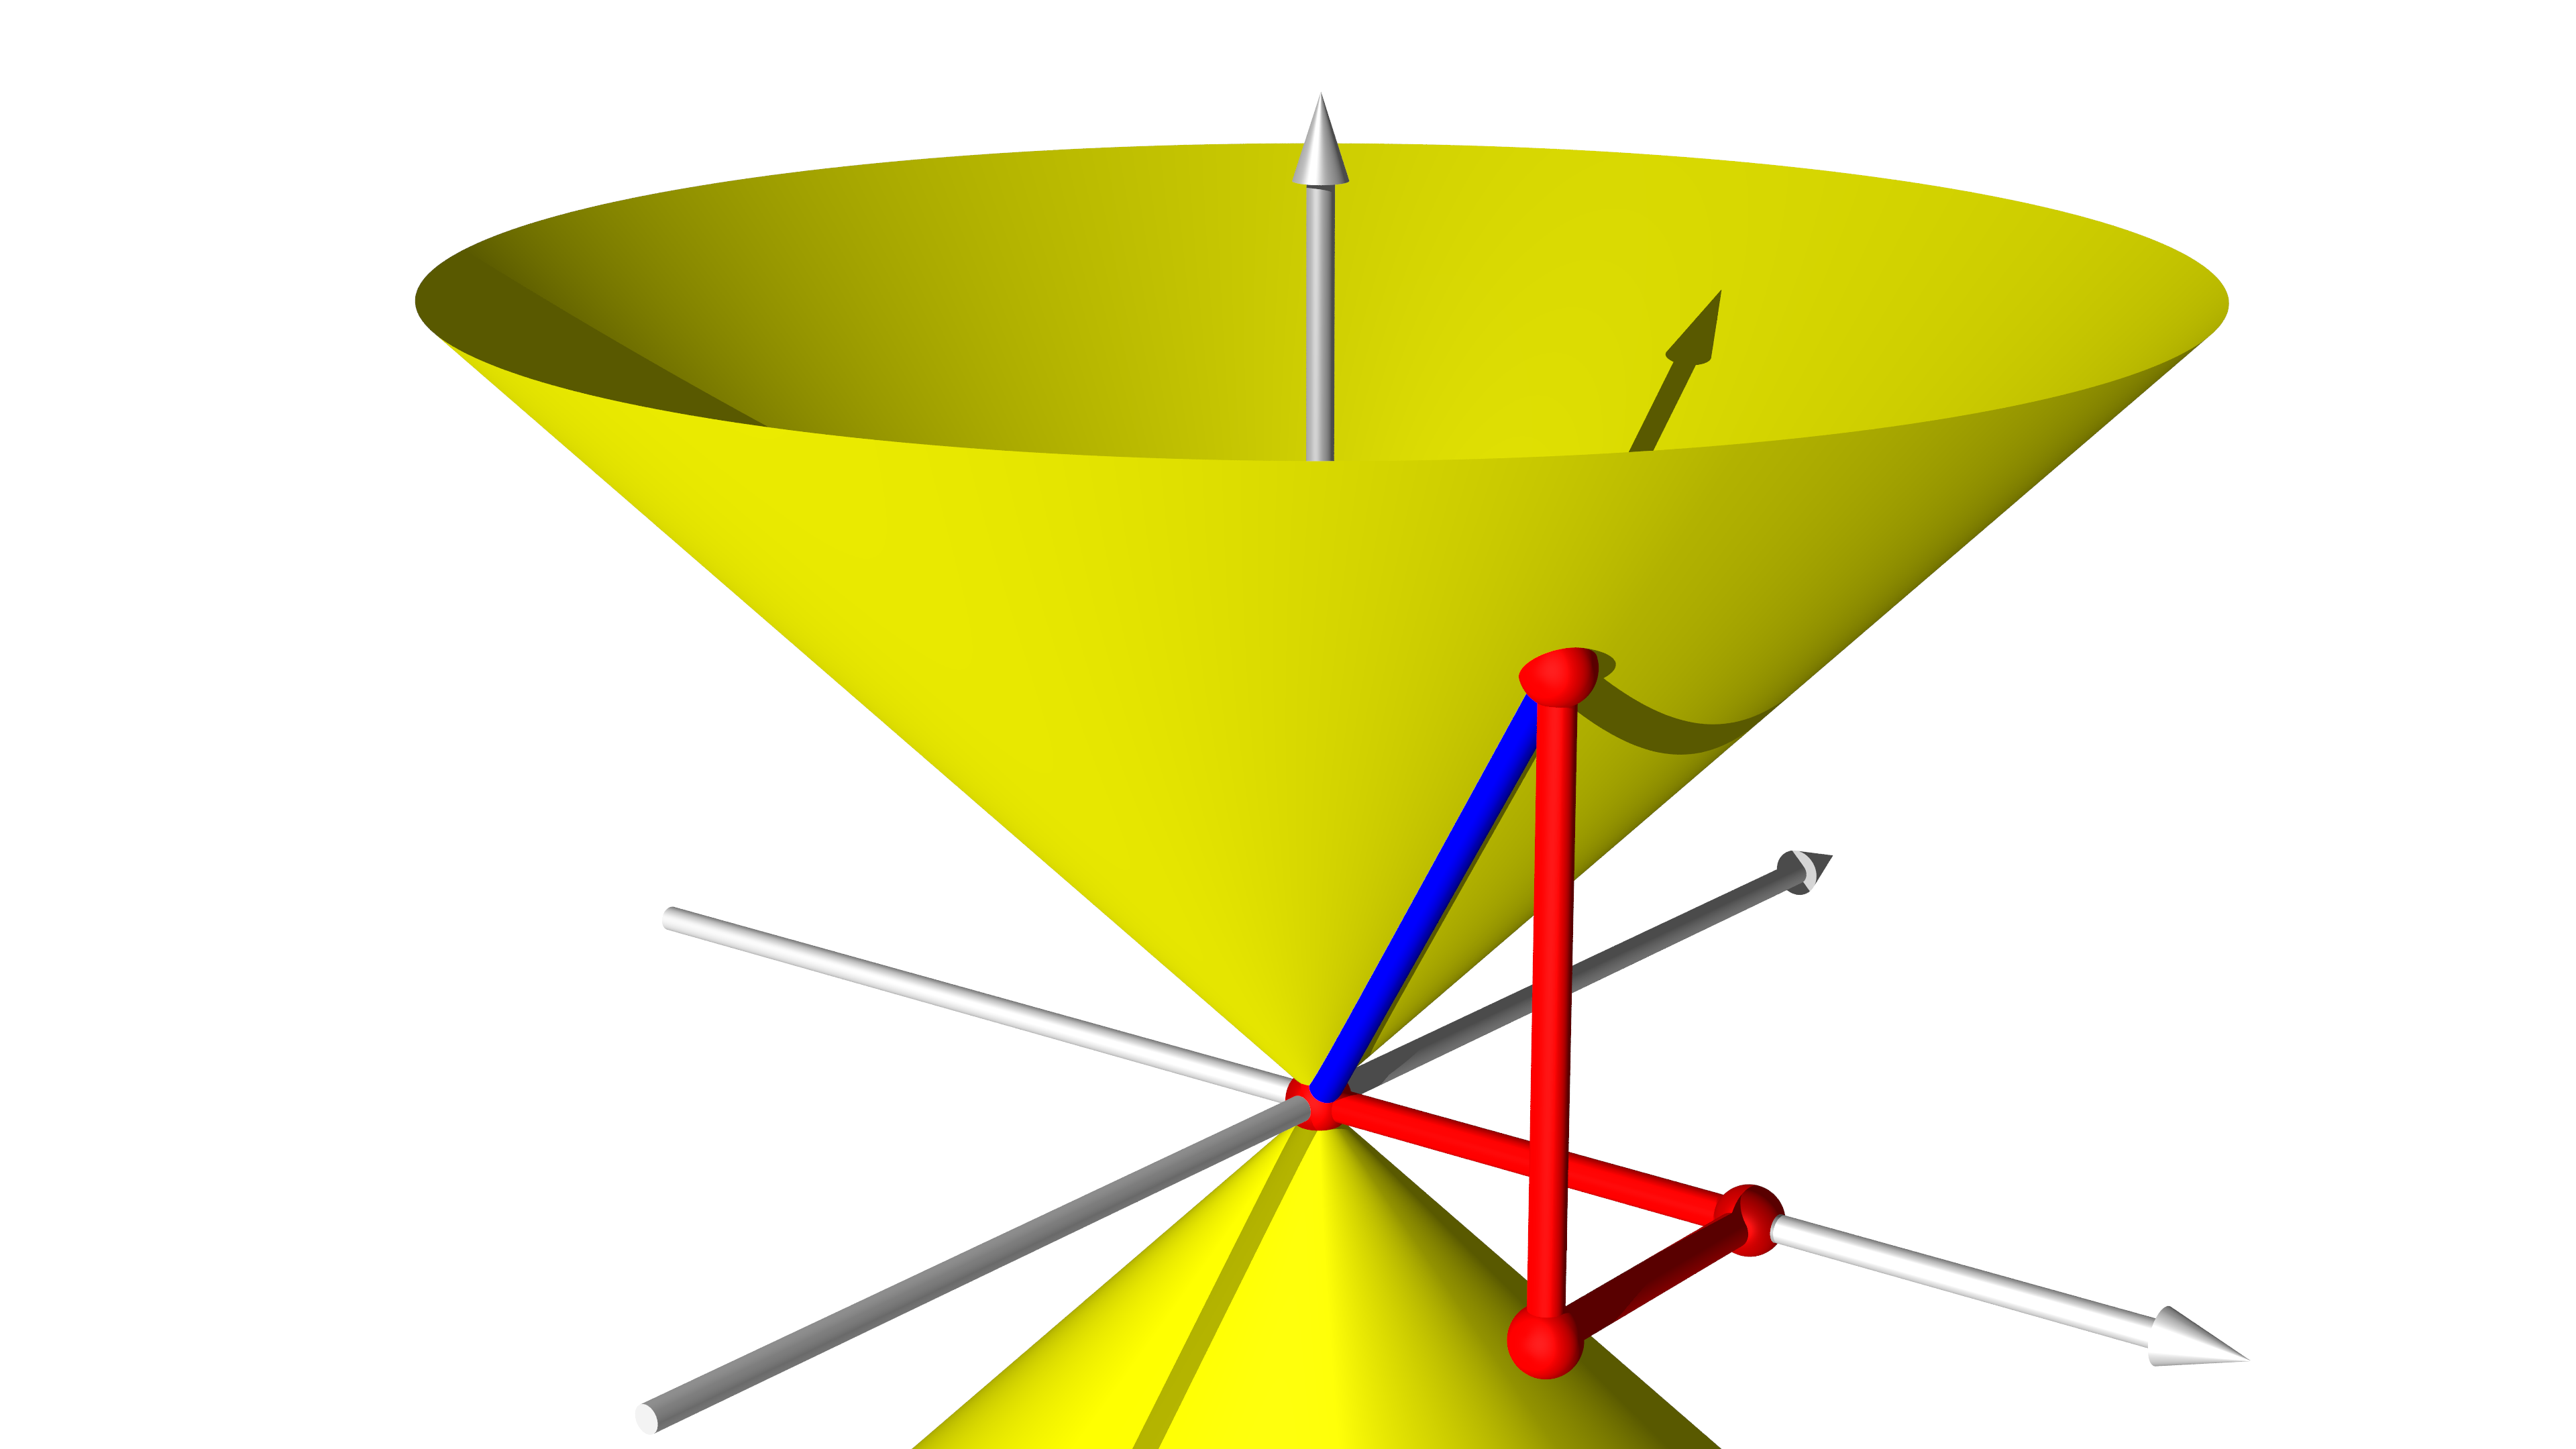
\includegraphics{chapters/tikz/lichtkegel.pdf}
\caption{Lichtkegel in Finkelstein-Koordinaten.
\label{skript:kruemmung:fig:lichtkegel-finkel}}
\end{figure}
In Finkelstein-Koordinaten verschwindet die Singularität bei $r=r_g$,
es sollte daher auch einfacher werden, die Bahn eines radial ins
Zentrum des Feldes stürzenden Teilchens zu berechnen.
Dazu können wir die Winkel-Koordinaten $\vartheta$ und $\varphi$
vernachlässigen und nur mit den Koordinaten $\tau$ und $R$ und der
Metrik
\[
ds^2
=
-c^2 \,d\tau^2
+r _g^{\frac23}\biggl(\frac32(R-c\tau)\biggr)^{\frac23}\,dR^2
\]
arbeiten.
\rhead{Absturz ins Zentrum}
Zur Berechnung der Bahnkurven brauchen wir die Christoffel-Symbole
2.~Art.
Die Berechnung mit Maxima ergibt
\begin{align*}
\Gamma^1_{11} &= 0,&
\Gamma^1_{12} &= 0,&
\Gamma^1_{21} &= 0,&
\Gamma^1_{22} &= \frac{2^{\frac23}r_g^{\frac23}}{(3(R-c\tau))^{\frac53}},\\
\Gamma^2_{11} &= 0,&
\Gamma^2_{12} &= \frac1{3(R-c\tau)},&
\Gamma^2_{21} &= \frac1{3(R-c\tau)},&
\Gamma^2_{22} &= -\frac1{3(R-c\tau)}.
\end{align*}
Wir beschreiben die Bahn eines Teilchens, welches sich in diesem Feld
radial bewegt, mit den Funktionen $\tau(s)$ und $R(s)$.
Wir untersuchen ein Teilchen, welches beim Punkt $\tau(0)=0$ und $R(0)=R_0$
mit Anfangsrichtung $\dot\tau(0)=1$ und $\dot R(0)=0$ in das Gravitationsfeld
stürzt.
Die Geodätengleichungen lauten
\begin{align*}
\frac{d^2\tau(s)}{ds^2}
&=
\Gamma^1_{22}\biggl(\frac{dR(s)}{ds}\biggr)^2,
\\
\frac{d^2R(s)}{ds^2}
&=
\Gamma^2_{12}\frac{d\tau(s)}{ds}\frac{dR(s)}{ds}
+
\Gamma^2_{22}\biggl(\frac{dR(s)}{ds}\biggr)^2.
\end{align*}
Da für die Anfangsbedinung $\dot R=0$ ist und auf der rechten Seite
$\dot R$ in jedem Term vorkommt, folgt aus der zweiten Gleichung
$\ddot R=0$, $\dot R$ kann sich also nicht ändern.
Wenn aber $\dot R=0$ für alle Werte von $s$, dann ist nach der ersten
Gleichung auch $\ddot \tau=0$ und damit $\dot \tau=1$.
Die Lösungskurve ist also $R=R_0$ und $\tau=s$, rot dargestellt in
Abbildung~\ref{skript:kruemmung:fig:absturz}
und
Abbildung~\ref{skript:kruemmung:fig:lichtkegel-finkel}.

Mit Hilfe der Formel~\eqref{skript:kruemmung:finkelsteinr}
kann man damit auch $r$ in Abhängigkeit von $\tau$ für den radialen Absturz
angeben:
\[
r(\tau)=\biggl(\frac32(R_0-c\tau)\biggr)^{\frac23}r_g^{\frac13}.
\]
Die Weltlinie eines radialen Absturzes in diesen Koordinaten ist in
Abbildung~\ref{skript:kruemmung:fig:blackhole} dargestellt.

\section{Ereignishorizont%
\label{skript:section:ereignishorizont}}
\rhead{Ereignishorizont}
Wir betrachten wieder die
Schwarzschild-Metrik~\eqref{skript:kruemmung:schwarzschildmetrik}
und möchten genauer verstehen, was bei $r=r_g$ passiert.
Dazu überlegen wir uns, wie ein Geodäte eines realen Teilchens 
aussieht.
Wir wissen, dass reale Teilchen sich entlang von Weltlinien bewegen müssen,
deren Tangentialvektor zeitartig ist.
Ein Teilchen in Ruhe hat zum Beispiel $\dot r=0$, $\dot \vartheta=0$ und
$\dot\varphi=0$, einzig $\dot t\ne 0$.
Da der Koeffizient von $dt^2$
\[
-\biggl(1-\frac{r_g}{r}\biggr)
\quad
\begin{cases}
<0&\qquad\text{für}\quad r > r_g
\\
>0&\qquad\text{für}\quad r < r_g
\end{cases}
\]
für $r>r_g$
negativ ist folgt, dass es tatsächlich möglich ist, dass sich ein Teilchen
in festem Abstand vom Zentrum aufhalten kann.
Sobald aber $r<r_g$ ist, ist der Koeffizient von $dt^2$ positiv,
fester Abstand vom Zentrum ist nicht mehr möglich.

Für $r<r_g$ wechselt aber auch das Vorzeichen des Koeffizienten
\[
\frac1{\displaystyle1-\frac{r_g}{r}}
\quad
\begin{cases}
>0&\qquad \text{für}\quad r>r_g
\\
<0&\qquad \text{für}\quad r<r_g
\end{cases}
\]
von $dr^2$, damit wird plötzlich der Vektor $\dot t=0$, $\dot r\ne 0$,
$\dot\vartheta=\dot\varphi=0$ zeitartig.
Sobald ein Teilchen sich innerhalb des Radius $r_g$ befindet, kann
sein Radius nur noch abnehmen.
Die Berechnung der Bahn eines solchen Teilchens zeigt auch, dass
es unausweichlich in endlicher Zeit ins Zentrum stürzen wird.
In Abbildung~\ref{skript:kruemmung:fig:lichtkegel-finkel} erkennt 
man dies daran, dass der Lichtkegel beim Überschreiten von $r=r_g$
so eng wird, dass zeitartige Vektoren die Linie $r=r_g$ in umgekehrter
Richtung nicht mehr kreuzen können.

\begin{figure}
\centering
%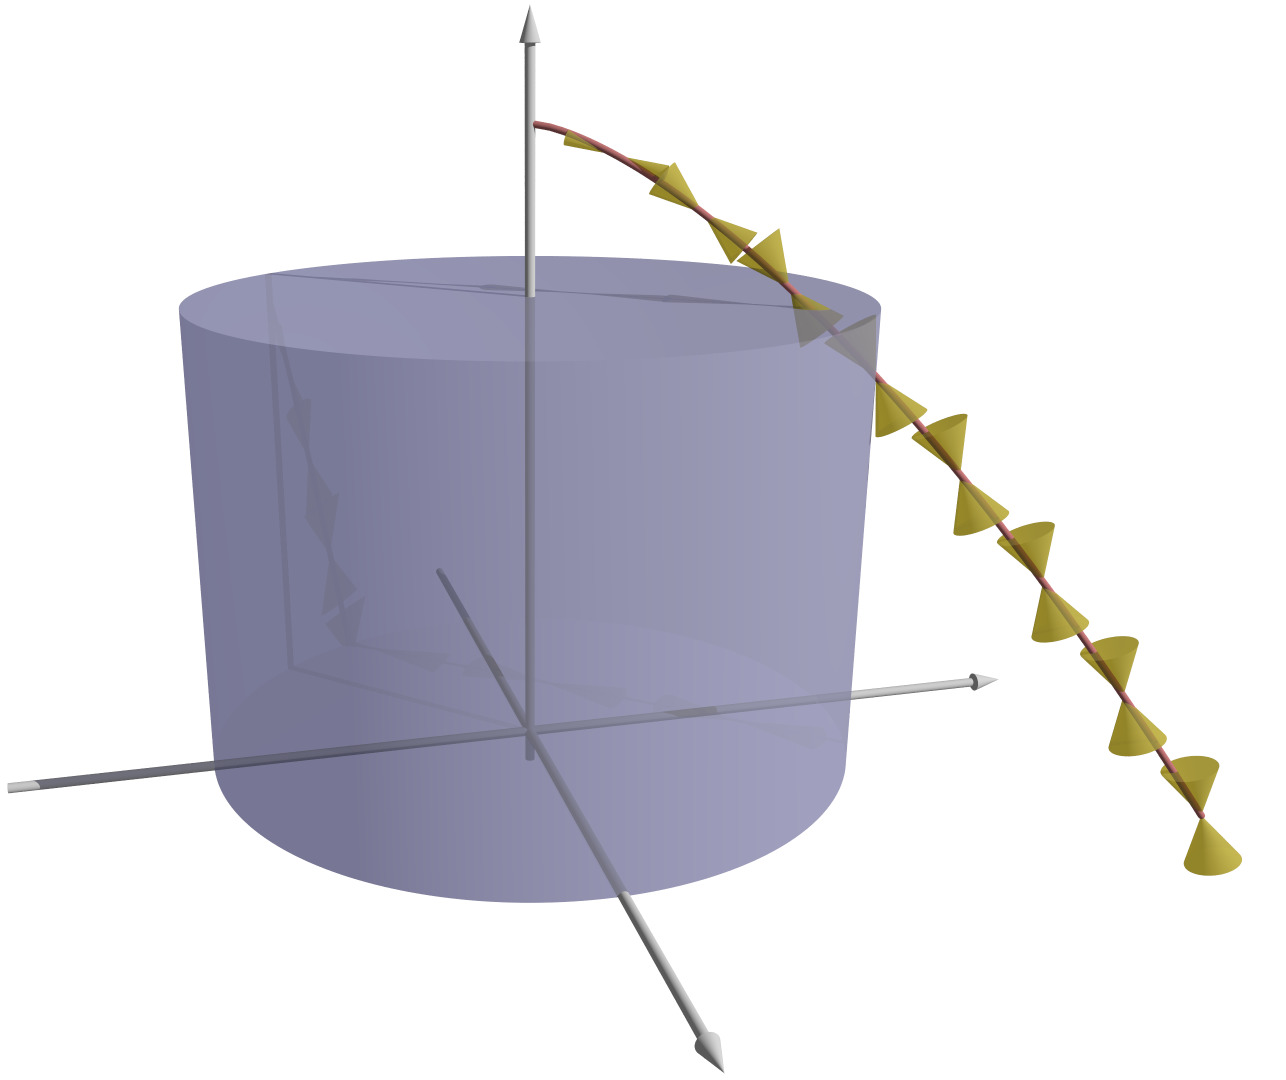
\includegraphics[width=\hsize]{chapters/3d/blackhole.jpg}
\begin{tikzpicture}[]
\coordinate (O) at (0,0);
\node at (0,0) {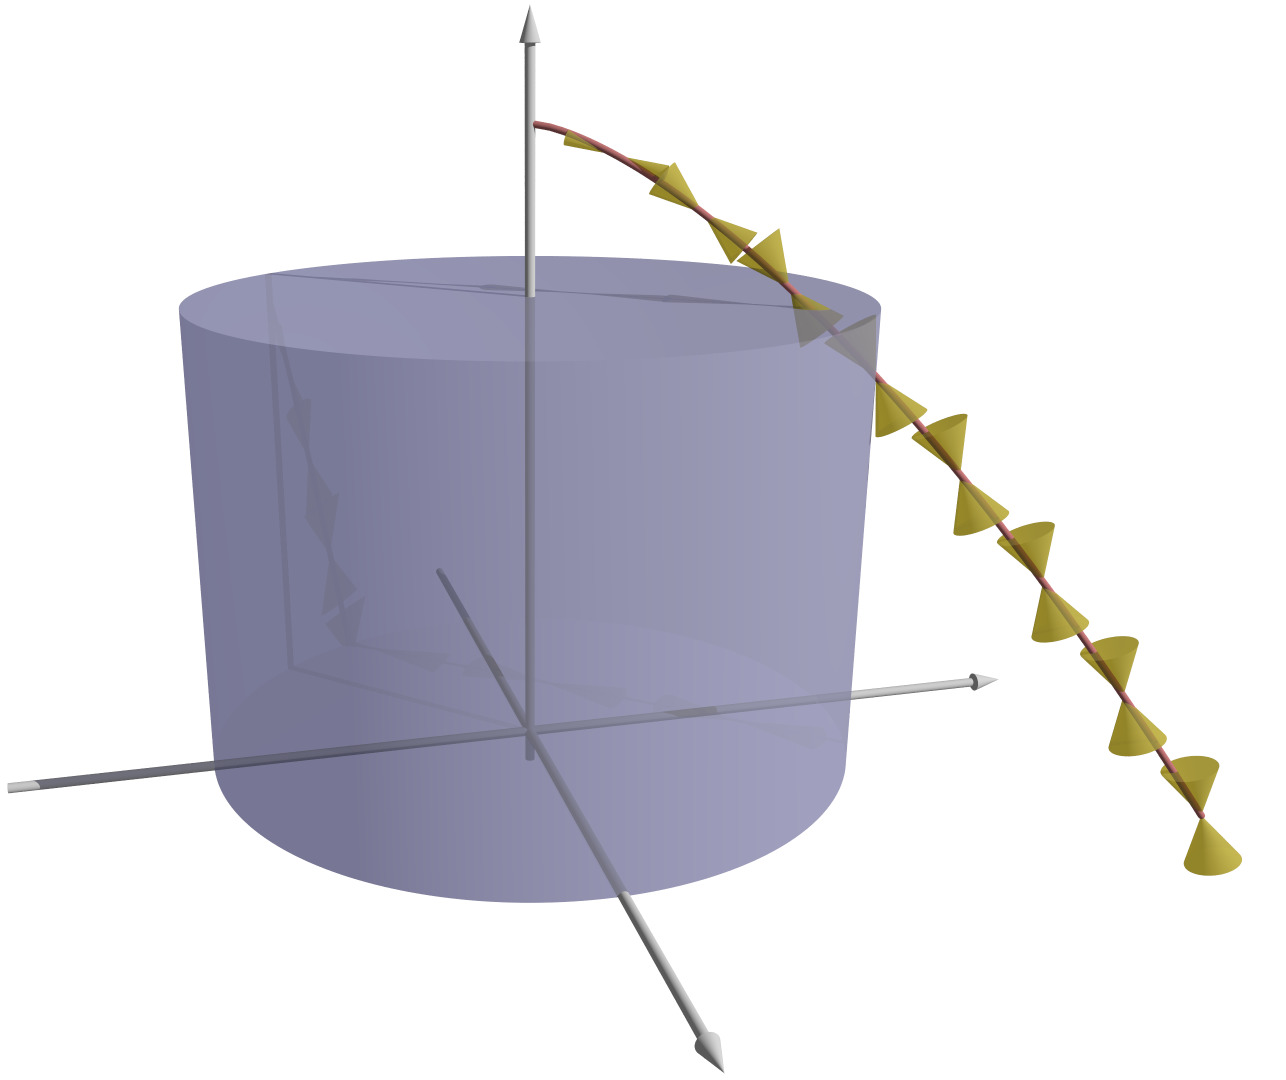
\includegraphics[width=\hsize]{chapters/3d/blackhole.jpg}};
\node at (4.1,-1.5) {$y$};
\node at (1.1,-5.5) {$x$};
\node at (-0.9,5.8) {$\tau$};
\end{tikzpicture}
\caption{Absturz eines Teilchens durch den Ereignishorizont in
$(\tau,r,\varphi)$-Koordinaten.
Sobald das Teilchen durch den Ereignishorizont gefallen ist,
befindet sich der ganze zukünftige Lichtkegel eines Teilchens 
immer vollständig im Inneren des Gebietes $r<r_g$.
\label{skript:kruemmung:fig:blackhole}}
\end{figure}


\section{Was spürt man am Ereignishorizont?%
\label{skript:section:wasspuertman}}
\rhead{Was spürt man am Ereignishorizont?}
Der Riemannsche Krümmungstensor gibt an, wie schnell Geodäten von Teilchen
wegen unterschiedlicher Gravitationswirkung sich voneinander entfernen.
Er bestimmt also die sogenannten Gezeitenkräfte, die ein Astronaut spürt,
der in diesem Gravitationsfeld abstürzt.
\index{Gezeitenkräfte}%
Die Berechnung des Riemann-Tensors mit Maxima ergibt aber:
\begin{align*}
R_{1212}&=-\frac{r_g}{r^3},
\end{align*}
die Gezeitenkräfte in radialer Richtung werden für den Astronauten
zwar immer grösser, er wird in die Länge gezogen und schliesslich 
zerrissen, darüber hinaus aber spürt er bei $r=r_g$ nichts Besonderes.
\index{Ereignishorizont}%

\section{Bedeutung von $r_g$%
\label{skript:schwarzschild:rg}}
\rhead{Bedeutung von $r_g$}
In Abschnitt~\ref{skript:section:ereignishorizont} haben wir gefunden,
dass sich bei der Koordinaten $r=r_g$ der Ereignishorizont befindet.
Es ist auch einigermassen klar, dass dieser Radius $r_g$ mit der
Masse des Objektes zusammenhängen muss.
Doch wie gross ist eigentlich der Gravitations-Radius $r_g$ verschiedener
uns umgebender Himmelskörper? Kann es überhaupt einen Körper geben, der
so dicht ist, dass er kleiner ist als sein Gravitationsradius?

In grosser Entfernung $r \gg r_g$ vom Zentrum ist die Metrik fast flach,
das Feld ist dort sehr schwach.
Durch Vergleich mit der Näherung~\eqref{skript:gravitation:naeherung}
finden wir
\[
\frac{r_g}{r} = \frac{2MK}{c^2r}
\qquad\Rightarrow\qquad
r_g=\frac{2MK}{c^2}.
\]
Der Radius $r_g=2MK$ heisst der {\em Gravitationsradius} oder 
\index{Gravitationsradius}%
{\em Schwarzschild-Radius}.
\index{Schwarzschild-Radius}%
Der numerische Zusammenhang zwischen Masse und Gravitationsradius
in SI-Einheiten ist
\[
r_g = \frac{2K}{c^2}M
=
2\cdot 6.67408\cdot10^{-11}
\frac{\text{m}^3}{\text{kg}\cdot\text{s}^2}
\cdot
\frac1{(2.99792458\cdot 10^{8}\frac{\text{m}}{\text{s}})^2}\cdot M
=
1.485183\cdot 10^{-27}\frac{\text{m}}{\text{kg}}\cdot M.
\]
Der Gravitationsradius der Sonne ist 
\begin{align*}
r_g
&=
1.485183\cdot 10^{-27}\frac{\text{m}}{\text{kg}}M
=
2.95403\cdot 10^{3}\text{m}
=
2.954\,\text{km}.
\end{align*}
Könnte man die Sonne auf eine Kugel mit einem Radius kleiner als 2.954km
komprimieren, würde sie zu einem schwarzen Loch und wäre nicht mehr
sichtbar.
Der Gravitationsradius der Erde ist dagegen viel kleiner:
\[
r_g
=
1.485183\cdot 10^{-27}\frac{\text{m}}{\text{kg}}M
\cdot
5.972\cdot 10^{24}\text{m}
=
8.87\cdot 10^{-3}\text{m}
=
8.87\text{mm}.
\]
Der Gravitationsradius ist also kleiner als ein Zentimeter.

%
% s-perihel.tex -- relativistische Periheldrehung, numerisch berechnet
%
% (c) 2017 Prof Dr Andreas Müller, Hochschule Rappersiwl
%

\section{Periheldrehung}
\rhead{Periheldrehung}
\begin{figure}
\centering
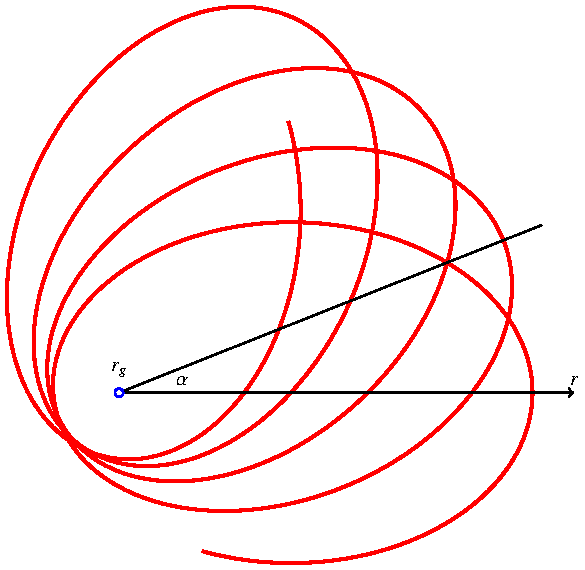
\includegraphics{chapters/tikz/orbit.pdf}
\caption{Periheldrehung um den Winkel $\alpha$ in jedem Umlauf um den
Zentralkörper in einer Schwarzschild-Metrik mit Anfangsbedingungen
\label{skript:schwarzschild:anfangsbedingung:normal}.
\label{skript:schwarzschild:perihelorbit}}
\end{figure}
Das erste Keplersche Gesetz sagt, dass ein Planet sich auf einer
Ellipsenbahn bewegt.
Die Newtonsche Gravitationstheorie bestätigt dies, die Differentialgleichungen
für das Zweikörperproblem sind in geschlossener Form lösbar.
Insbesondere zeigt die Richtung zum sonnennächsten Punkt, dem Perihel,
immer in die gleiche Richtung.
Für die Merkurbahn wurde jedoch eine Abweichung festgestellt, die
Perihelrichtung dreht sich mit der Zeit um die Sonne.
Einen Teil dieser Drehung konnte mit der newtonschen Theorie erklärt werden.
So führen zum Beispiel die Abplattung der Sonne und die Störungen durch
andere Planeten zu einem solchen Effekt.
Von den gemessenen $571.91''$ Periheldrehung des Merkur pro Jahrhundert
verblieben jedoch $43.11''$ pro Jahrhundert, die die Newtonsche
Theorie nicht erklären konnte.


Schon in seinem ursprünglichen Entwurf der allgemeinen Relativitätstheorie
hat Einstein die durch die Abweichung von der Newtonschen Theorie
verursachte Periheldrehung der Merkurbahn berechnet und gute Übereinstimmung
mit der bekannten Drehung gefunden.
Damit hat er bereits selbst eine erste experimentelle Bestätigung
der Theorie gegeben.

Um den Effekt überhaupt darstellen zu können, muss die Bahn sehr nahe
am Zentralkörper vorbeiführen, der nächste Punkt, das Apastron darf
also nur wenige Gravitationsradien entfernt sein.
In Abbildung~\ref{skript:schwarzschild:perihelorbit} ist die
Umlaufbahn eines Körpers dargestellt, dessen Apastron-Entfernung
$100 r_g$ ist und der sich im Periastron auf etwa $20r_g$ 
nähert.
Die Apsidenlinie dreht sich hier in jedem Umlauf um $\alpha = 21.61^\circ$.
Ziel dieses Abschnittes ist zu zeigen, wie die Periastron-Drehung
in einer Schwarzschild-Metrik numerisch berechnet werden kann.
Es geht dabei nicht darum, den exakten Wert für die Periheldrehung
des Merkur zu bestimmen,
sondern nur zu zeigen, dass die allgemeine Relativitätstheorie
qualititativ einen solchen Effekt vorhersagt.

\subsection{Geodätengleichung für die Schwarzschild-Metrik}
\label{skript:schwarzschild:geodaetengleichung}
%(%i5) 		        ratsimp(Christoffel2(1, 1, 1))
%(%o5) 				       0
%(%i6) 		        ratsimp(Christoffel2(1, 1, 2))
%				       rg
%(%o6) 			        - -------------
%					      2
%				  2 r rg - 2 r
%(%i7) 		        ratsimp(Christoffel2(1, 1, 3))
%(%o7) 				       0
%(%i8) 		        ratsimp(Christoffel2(1, 1, 4))
%(%o8) 				       0
%(%i9) 		        ratsimp(Christoffel2(1, 2, 2))
%(%o9) 				       0
%(%i10) 		        ratsimp(Christoffel2(1, 2, 3))
%(%o10) 				       0
%(%i11) 		        ratsimp(Christoffel2(1, 2, 4))
%(%o11) 				       0
%(%i12) 		        ratsimp(Christoffel2(1, 3, 3))
%(%o12) 				       0
%(%i13) 		        ratsimp(Christoffel2(1, 3, 4))
%(%o13) 				       0
%(%i14) 		        ratsimp(Christoffel2(1, 4, 4))
%(%o14) 				       0
%(%i15) 		        ratsimp(Christoffel2(2, 1, 1))
%				     2
%				   rg  - r rg
%(%o15) 				 - ----------
%					 3
%				      2 r
%(%i16) 		        ratsimp(Christoffel2(2, 1, 2))
%(%o16) 				       0
%(%i17) 		        ratsimp(Christoffel2(2, 1, 3))
%(%o17) 				       0
%(%i18) 		        ratsimp(Christoffel2(2, 1, 4))
%(%o18) 				       0
%(%i19) 		        ratsimp(Christoffel2(2, 2, 2))
%				      rg
%(%o19) 				 -------------
%					     2
%				 2 r rg - 2 r
%(%i20) 		        ratsimp(Christoffel2(2, 2, 3))
%(%o20) 				       0
%(%i21) 		        ratsimp(Christoffel2(2, 2, 4))
%(%o21) 				       0
%(%i22) 		        ratsimp(Christoffel2(2, 3, 3))
%(%o22) 				    rg - r
%(%i23) 		        ratsimp(Christoffel2(2, 3, 4))
%(%o23) 				       0
%(%i24) 		        ratsimp(Christoffel2(2, 4, 4))
%					 2
%(%o24) 			     (rg - r) sin (theta)
%(%i25) 		        ratsimp(Christoffel2(3, 1, 1))
%(%o25) 				       0
%(%i26) 		        ratsimp(Christoffel2(3, 1, 2))
%(%o26) 				       0
%(%i27) 		        ratsimp(Christoffel2(3, 1, 3))
%(%o27) 				       0
%(%i28) 		        ratsimp(Christoffel2(3, 1, 4))
%(%o28) 				       0
%(%i29) 		        ratsimp(Christoffel2(3, 2, 2))
%(%o29) 				       0
%(%i30) 		        ratsimp(Christoffel2(3, 2, 3))
%				       1
%(%o30) 				       -
%				       r
%(%i31) 		        ratsimp(Christoffel2(3, 2, 4))
%(%o31) 				       0
%(%i32) 		        ratsimp(Christoffel2(3, 3, 3))
%(%o32) 				       0
%(%i33) 		        ratsimp(Christoffel2(3, 3, 4))
%(%o33) 				       0
%(%i34) 		        ratsimp(Christoffel2(3, 4, 4))
%(%o34) 			    - cos(theta) sin(theta)
%(%i35) 		        ratsimp(Christoffel2(4, 1, 1))
%(%o35) 				       0
%(%i36) 		        ratsimp(Christoffel2(4, 1, 2))
%(%o36) 				       0
%(%i37) 		        ratsimp(Christoffel2(4, 1, 3))
%(%o37) 				       0
%(%i38) 		        ratsimp(Christoffel2(4, 1, 4))
%(%o38) 				       0
%(%i39) 		        ratsimp(Christoffel2(4, 2, 2))
%(%o39) 				       0
%(%i40) 		        ratsimp(Christoffel2(4, 2, 3))
%(%o40) 				       0
%(%i41) 		        ratsimp(Christoffel2(4, 2, 4))
%				       1
%(%o41) 				       -
%				       r
%(%i42) 		        ratsimp(Christoffel2(4, 3, 3))
%(%o42) 				       0
%(%i43) 		        ratsimp(Christoffel2(4, 3, 4))
%				  cos(theta)
%(%o43) 				  ----------
%				  sin(theta)
%(%i44) 		        ratsimp(Christoffel2(4, 4, 4))
%(%o44) 				       0
%
Für die Geodätengleichungen brauchen wir die Christoffsymbole 
für die Schwarzschild Metrik.
Mit Maxima kann man die folgenden nicht verschwindenden
$\Gamma^\mu_{\alpha\beta}$ 
finden:
\begin{align*}
%(%i6) 		        ratsimp(Christoffel2(1, 1, 2))
%				       rg
%(%o6) 			        - -------------
%					      2
%				  2 r rg - 2 r
\Gamma^0_{01}
&=
\frac{1}{1-\displaystyle\frac{r_g}{r}}
\frac{r_g}{r}
\frac{1}{2r}
\\
%(%i15)                  ratsimp(Christoffel2(2, 1, 1))
%                                     2
%                                  rg  - r rg
%(%o15)                          - ----------
%                                         3
%                                      2 r
\Gamma^1_{00}
&=
\biggl(1-\displaystyle\frac{r_g}{r}\biggr)
\frac{r_g}{r}
\frac{1}{2r}
&
%(%i19)                  ratsimp(Christoffel2(2, 2, 2))
%                                      rg
%(%o19)                           -------------
%                                             2
%                                 2 r rg - 2 r
\Gamma^1_{11}
&=
-\frac1{1-\displaystyle\frac{r_g}{r}}
\frac{r_g}{r}
\frac{1}{2r}
&
%(%i22) 		        ratsimp(Christoffel2(2, 3, 3))
%(%o22) 				    rg - r
\Gamma^1_{22}
&=
r_g-r
&
%(%i24)                  ratsimp(Christoffel2(2, 4, 4))
%                                         2
%(%o24)                       (rg - r) sin (theta)
\Gamma^1_{33}
&=
(r_g-r)\sin^2\vartheta
\\
%(%i30)                  ratsimp(Christoffel2(3, 2, 3))
%                                       1
%(%o30)                                 -
%                                       r
\Gamma^2_{12}
&=
\frac1r
&
%(%i34) 		        ratsimp(Christoffel2(3, 4, 4))
%(%o34) 			    - cos(theta) sin(theta)
\Gamma^2_{33}
&=
-\cos\vartheta \sin\vartheta
\\
%(%i41)                  ratsimp(Christoffel2(4, 2, 4))
%                                       1
%(%o41)                                 -
%                                       r
\Gamma^3_{13}
&=
\frac1r
&
%(%i43)                  ratsimp(Christoffel2(4, 3, 4))
%                                  cos(theta)
%(%o43)                            ----------
%                                  sin(theta)
\Gamma^3_{23}
&=
\cot\vartheta
\end{align*}
Wir betrachten jetzt eine Geodäte, die mit dem Parameter $s$ parametrisiert ist.
In allgemeiner Form schreiben wir dafür $x^\mu(s)$, im speziellen
Koordinatensystem der Schwarzschild-Metrik ist
\[
\begin{aligned}
x^0(s)&=t(s),
&
x^1(s)&=r(s),
&
x^2(s)&=\vartheta(s),
&
x^3(s)&=\varphi(s).
\end{aligned}
\]
Die zugehörigen Geodätengleichungen sind
\begin{align*}
\ddot t(s)
&=
-\frac{1}{1-\displaystyle\frac{r_g}{r}}\frac{r_g}{r}\frac{1}{r}\dot t(s)\,\dot r(s)
\\
\ddot r(s)
&=
-\biggl(1-\frac{r_g}{r}\biggr)\frac{r_g}{r}\frac1{2r}\dot t(s)^2
+\frac{1}{1-\displaystyle\frac{r_g}{r}} \frac{r_g}{r}\frac1{2r}\dot r(s)^2
-(r_g-r)\dot \vartheta(s)^2 + (r_g-r)\sin^2 \vartheta \cdot \dot \varphi(s)^2
\\
\ddot \vartheta(s)
&=
-\frac{2}{r} \dot r(s)\, \dot \vartheta(s)
+\cos\vartheta\sin\vartheta \cdot \dot\varphi(s)^2
\\
\ddot \varphi(s)
&=
-\frac{2}{r} \dot r(s)\,\dot \varphi(s)
-2\cot\vartheta \cdot \dot r(s)\,\dot\varphi(s)
\end{align*}
Darin ist natürlich $r$ in den Koeffizienten jeweils als $r(s)$ zu lesen.

Wir wollen eine Bahn in der Ebene $\vartheta=\frac{\pi}2$ berechnen.
Setzen wir diesen Wert ein, verschwinden auch noch die Terme, die
$\cos\vartheta$ enthalten.
Es bleiben nur noch
\begin{equation}
\begin{aligned}
\Gamma^0_{01}
&=
\frac{1}{1-\displaystyle\frac{r_g}{r}}
\frac{r_g}{r}
\frac{1}{2r}
\\
\Gamma^1_{00}
&=
\biggl(1-\displaystyle\frac{r_g}{r}\biggr)
\frac{r_g}{r}
\frac{1}{2r}
&
\Gamma^1_{11}
&=
-\frac1{1-\displaystyle\frac{r_g}{r}}
\frac{r_g}{r}
\frac{1}{2r}
&
\Gamma^1_{22}
&=
r_g-r
&
\Gamma^1_{33}
&=
r_g-r
\\
%(%i30)                  ratsimp(Christoffel2(3, 2, 3))
%                                       1
%(%o30)                                 -
%                                       r
\Gamma^2_{12}
&=
\frac1r
\\
%(%i41)                  ratsimp(Christoffel2(4, 2, 4))
%                                       1
%(%o41)                                 -
%                                       r
\Gamma^3_{13}
&=
\frac1r
\end{aligned}
\label{skript:schwarzschild:christoffelaequator}
\end{equation}
Hat eine Geodäte eine Anfangsgeschwindigkeit in der Äquatorebene, dann
ist $\dot x^3(0) = \dot\vartheta(0)=0$.
Die Geodätengleichung für $\ddot \vartheta$ ist dann
\[
\ddot \vartheta(s)
=
\ddot x^2(s)
=
\Gamma^2_{12}\dot r(s)\dot \vartheta(s),
\]
insbesondere bleibt $\dot\vartheta(s)=0$ entlang der ganzen Geodäten.
Die Geodäte wird daher die Äquatorebenen nicht verlassen.
Da man das Koordinatensystem immer so wählen kann, dass $\dot\vartheta(0)=0$
ist, kann man ganz allgemein sagen, dass Geodäten in einer Schwarzschild-Metrik
in einer Ebene liegen.
Man hätte also auch von Anfang an in Polarkoordinaten rechnen können.

Die vereinfachten Christoffelsymbole für die Äquatorebene
\eqref{skript:schwarzschild:christoffelaequator}
führen auch auf vereinfachte Geodätengleichungen, wenn wir $\dot\vartheta(s)=0$
berücksichtigen.
Wir erhalten
\begin{align*}
\ddot t(s)
&=
-\frac{1}{1-\displaystyle\frac{r_g}{r}}\frac{r_g}{r}\frac{1}{r}\dot t(s)\,\dot r(s)
\\
\ddot r(s)
&=
-\biggl(1-\frac{r_g}{r}\biggr)\frac{r_g}{r}\frac1{2r}\dot t(s)^2
+\frac{1}{1-\displaystyle\frac{r_g}{r}} \frac{r_g}{r}\frac1{2r}\dot r(s)^2
- (r_g-r) \dot\varphi(s)^2
\\
\ddot \vartheta(s)
&=
0
\\
\ddot \varphi(s)
&=
-\frac2r \dot r(s)\,\dot\varphi(s)
\end{align*}
Diese Gleichungen lassen sich nicht in geschlossener Form integrieren.
Durch numerische Lösung für geeignete Anfangswerte kann man jedoch die
Drehung der Apsidenlinie sichtbar machen.

\subsection{Numerische Lösung}
Im Repository zu befinden sich einige Octave-Programme, mit denen man
die Geodäten in einer Schwarzschild-Metrik berechnen kann.
Um zu etwas leichter verständlichen Zahlen zu kommen, rechnen wir
in diesen Programmen immer mit Masseinheiten so, dass $r_g=1$ ist,
d.~h.~der Gravitationsradius des Zentralkörpers ist die Längeneinheit,
und $c=1$, d.~h.~$r_g/c$ ist die Zeiteinheit.

Der Parameter $s$ der Geodätengleichung ist genau dann die Eigenzeit,
wenn die Anfangsgeschwindigkeit den den Wert $-1$ hat.
In den Rechnungen muss daher die Anfangs-Vierergschwindigkeit $u^\mu$
so normiert werden, dass $g_\mu\nu u^\mu u^\nu=-1$ ist.

\subsubsection{Zustandsvektor}
Da die Geodätengleichungen Differentialgleichungen zweiter Ordnung sind,
muss man als Zustandsvektor den Vektor
\[
X=\begin{pmatrix}
t\\r\\\vartheta\\\varphi \\\dot t\\\dot r\\\dot \vartheta\\\dot\varphi
\end{pmatrix}
\]
verwenden.
Der Punkt bezeichnet darin die Ableitung nach dem Parameter $s$, der
wie gesagt bei geeigneter Normierung der Anfangsgeschwindigkeit mit
der Eigenzeit übereinstimmt.
Aus dem Vektor $X$ lässt sich jederzeit die Position und die
Vierergeschwindigkeit extrahieren.
Im File \text{geodesic.m} dienen dazu die Funktionen
\texttt{position} und \texttt{velocity}
\lstinputlisting[style=Octave]{chapters/listings/schwarzschild-extract.m}
Mit der Funktion \texttt{rescale} kann man im Vektor $X$ den
Geschwindigkeitsanteil um einen gegebenen Faktor strecken:
\lstinputlisting[style=Octave]{chapters/listings/schwarzschild-rescale.m}

\subsubsection{Metrik und Christoffel-Symbole}
Natürlich braucht man die Metrik, um den korrekten Wert zu berechnen.
Das File \texttt{geodesic.m} geht davon aus, dass die Funktion \texttt{metrik}
bereits definiert worden ist.
Für die Schwarzschild-Metrik geschieht dies im File
\texttt{christoffel-schwarzschild.m} mit der Funktion
\lstinputlisting[style=Octave]{chapters/listings/schwarzschild-metrik.m}
Diese Funktion berechnet das Skalarprodukt der Vektoren \texttt{u} und
\texttt{v} an der Stelle $x$.
Das File \texttt{christoffel-schwarzschild.m} definiert auch die Funktion
\texttt{christoffel}, die für jeden Index-Wert $\alpha$ die Matrix mit
den Einträgen $\Gamma^\alpha_{\mu\nu}$ für die Koordinatenwerte \texttt{x}
zurückgibt.
Für die Schwarzschild-Metrik ist dies
\lstinputlisting[style=Octave]{chapters/listings/schwarzschild-christoffel.m}

\subsubsection{Differentialgleichung}
Mit diesen zwei Funktionen ist es jetzt nicht mehr schwierig, eine Funktion
zu konstruieren, die Geodäten für jede beliebige Metrik berechnen kann.
Zunächst ist eine Funktion nötig, die die Differentialgleichung implementiert.
Für den Vektor $X$ geschrieben lautet diese
\[
\frac{dX}{ds}
=
\begin{pmatrix}
X_5\\X_6\\X_7\\X_8
\\
-\Gamma^1_{ij}X^iX^j\\
-\Gamma^2_{ij}X^iX^j\\
-\Gamma^3_{ij}X^iX^j\\
-\Gamma^4_{ij}X^iX^j
\end{pmatrix},
\]
wobei die Indizes $i$ und $j$ von $1$ bis $4$ laufen.
Da die Funktion \texttt{christoffel} die Werte der Christoffelsymbole
als Matrix $\Gamma^\alpha$ liefert, kann man für die Vierergschwindigkeit
$u$ die rechte Seite auch als $u^t \Gamma^\alpha u$ schreiben.
Die Differentialgleichung lässt sich daher in Octave durch die
Funktion
\lstinputlisting[style=Octave]{chapters/listings/geodesic-dgl.m}
implementieren.

Die Differentialgleichung lässt sich mit der Funktion \texttt{lsode}
lösen.
Die nötigen Schritt sind in der Funktion
\lstinputlisting[style=Octave]{chapters/listings/geodesic-solution.m}
zusammengefasst.

\subsubsection{Drehung der Apsidenlinie}
Die Drehung der Apsiden-Linie ist daran erkennbar, dass die Werte von
$\varphi(s)$, bei denen $r(s)$ sein Maximum und Minimum annimmt,
nicht jeweils um $\pi$ auseinanderliegen, sondern um einen grösseren
Wert.
Die Extrema von $r(s)$ sind erkennbar daran, dass $\dot r(s)=0$.
Man kann daher den Betrag der Drehung der Apsidenlinie dadurch
bestimmen, dass man numerisch die Nullstellen von $\dot r(s)$
bestimmt, und die zugehörigen Werte von $\varphi(s)$ ermittelt.

Die numerische Rechnung kann mit der Funktion \texttt{apsidbetween}
\lstinputlisting[style=Octave]{chapters/listings/apsiden-between.m}
durchgeführt werden.
Als Argument nimmt diese Funktion zwei Zustandsvektoren in der Form,
wie sie von der Funktion \texttt{geodesic}
zurückgegeben wird, also eine Zeile bestehend aus der aktuellen
Eigenzeit und den acht Komponenten des Zustandsvektors.
Die Funktion \texttt{apsidbetween} integriert dann auf Zeile~20
zehnmal kleinere Integrationsschritte in diesem Interval (und aus numerischen
Gründen noch etwas darüber hinaus) und sucht in den Zeilen 22 bis 25
das
erste Teilinterval, in dem das Vorzeichen von $\dot r(s)$ wechselt.
Mit den zugehörigen Zuständen wird \texttt{apsidbetween}
in Zeile 26
rekursiv augerufen, bis auf Zeile~6 die Differenz der Winkel $\phi(s)$ zwischen
den beiden Zuständen kleiner als $10^{-6}$ ist.

Der folgende Code berechnet die Werte von $\varphi(s)$ für alle
Extrema von $r(s)$ und ermittelt den Mittelwert:
\lstinputlisting[style=Octave]{chapters/listings/apsiden-winkel.m}

\subsubsection{Beispiel}
Die Umlaufbahn aus Abbildung~\ref{skript:schwarzschild:perihelorbit}
wurde mit den Anfangsbedingungen
\begin{equation}
\begin{aligned}
t(s)        &=\phantom{00}0.00000                    &\dot t(s)         &= 1.00577\\
r(s)        &=          100.00000                    &\dot r(s)         &= 0.00000\\
\vartheta(s)&=\phantom{00}1.57080=\textstyle\frac\pi2&\dot \vartheta(s) &= 0.00000\\
\varphi(s)  &=\phantom{00}0.00000                    &\dot \varphi(s)   &= 0.00038
\end{aligned}
\label{skript:schwarzschild:anfangsbedingung:normal}
\end{equation}
berechnet.
Es ergibt sich ein durchschnittlicher Wert von $21.6114^\circ$, um den die
Apsidenlinie vorrückt.

\subsubsection{Extreme Bahnen}
\begin{figure}
\centering
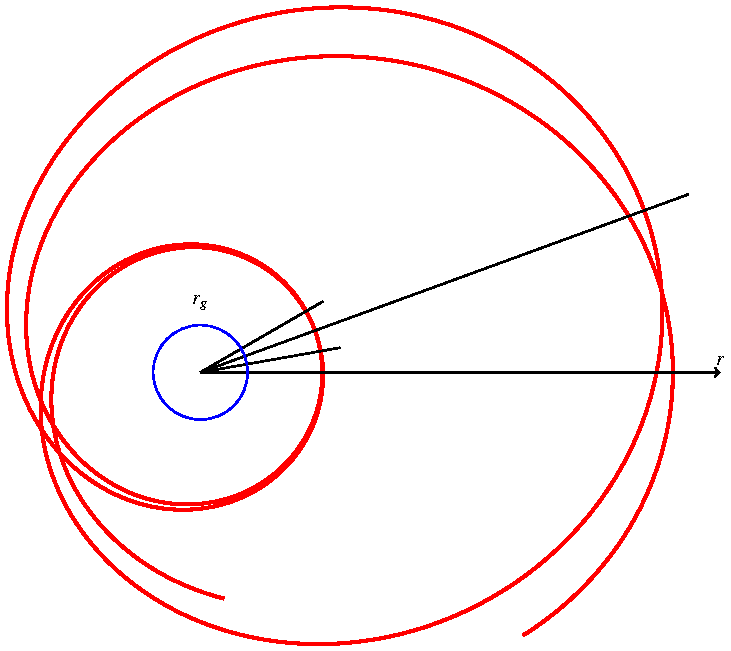
\includegraphics{chapters/tikz/orbit2.pdf}
\caption{Periheldrehung für eine Bahn, die sehr nahe an den Gravitationsradius
heranführt.
Anfangsbedingungen dieser Bahn sind
\eqref{skript:schwarzschild:anfangsbedingunge:extrem}.
\label{skript:schwarzschild:apside:extrem}}
\end{figure}
Bahnen, die sehr nahe an den Ereignishorizont heranführen, erfahren eine
noch viel deutlichere Drehung der Apsidenlinie.
In Abbildung~\ref{skript:schwarzschild:apside:extrem}
ist eine Bahn dargestellt, die sich auf weniger als $3r_g$ dem Zentralkörper
nähert.
Schon der Winkel $\varphi$ für das Perihel unterscheidet sich um um mehr
als $180^\circ$ vom Winkel $180^\circ$, der für eine Kepler-Bahn zu
erwarten wäre.
Die Anfangsbedingungen dieser Bahn sind
\begin{equation}
%    0.00000
%   10.00000
%    1.57080
%    0.00000
%    1.07220
%    0.00000
%    0.00000
%    0.01861
\begin{aligned}
t(s)        &=\phantom{0}0.00000                    &\dot t(s)         &= 1.07220\\
r(s)        &=          10.00000                    &\dot r(s)         &= 0.00000\\
\vartheta(s)&=\phantom{0}1.57080=\textstyle\frac\pi2&\dot \vartheta(s) &= 0.00000\\
\varphi(s)  &=\phantom{0}0.00000                    &\dot \varphi(s)   &= 0.01861
\end{aligned}
\label{skript:schwarzschild:anfangsbedingunge:extrem}
\end{equation}

%
% s-lichtablenkung.tex -- Lichtablenkung am Sonnenrand
%
% (c) 2017 Prof Dr Andreas Müller, Hochschule Rapperswil
%
\section{Lichtablenkung}
\rhead{Lichtablenkung}
\index{Lichtablenkung}
Die Ablenkung von Licht an der Sonne war eine der ersten Vorhersagen der
allgmeinen Relativitätstheorie.
Sie wurde 1918 während einer Sonnenfinsternisbeobachtung durch
Arthur Eddington nachgewiesen, und machte Einstein über Nacht zu einem Star.
\index{Eddington, Arthur}
Ziel dieses Abschnitts ist, die Bahn eines Lichstrahls numerisch
mit Hilfe der Schwarzschild Metrik zu berechnen.
Wir dürfen ohne Beschränkung der Allgemeinheit annehmen, dass der Lichtstrahl
sich in der $r$-$\varphi$-Ebene bewegt, dass also $\vartheta=\frac\pi2$ ist.
Wir arbeiten daher zur Vereinfachung in Polarkoordinaten mit der Metrik
\begin{equation}
ds^2
=
-\biggl(1-\frac{r_g}{r}\biggr)\,dt^2
+ \frac{1}{\displaystyle 1-\frac{r_g}{r}}\,dr^2
+ r^2\,d\varphi^2.
\label{skript:schwarzschild:metrik:polar}
\end{equation}

\subsection{Differentialgleichung}
Die gesuchte Kurve ist die Weltlinie eines Lichtstrahls, also ein Null-Geodäte. 
Zusätzlich zur Geodätengleichung erfüllt der Vektor der Vierergeschwindigkeit
auch noch die Bedingung $g_{\mu\nu}\dot x^\mu \dot x^\nu=0$.
Unter Verwendung von \eqref{skript:schwarzschild:metrik:polar}
wird daraus die Bedingung
\begin{equation}
\biggl(1-\frac{r_g}{r(s)}\biggr)\,\dot t(s)^2
=
\frac{1}{\displaystyle 1-\frac{r_g}{r(s)}}\,\dot r(s)^2
+ r(s)^2\dot \varphi(s)^2.
\label{skript:schwarzschild:dott2}
\end{equation}
Wir können mit Hilfe von \eqref{skript:schwarzschild:dott2}
den Term $\dot t(s)^2$ durch Ableitungen von $r(s)$ und $\varphi(s)$
ausdrücken und so die Variable $t$ eliminieren.
Auf diesem Weg versuchen wir ein Differentialgleichung für $r$
als Funktion von $\varphi$ zu finden.

Die Berechnungen auf dem Weg zu dieser Differentialgleichung sind
etwas mühsam.
Im Repository findet man das Maxima-Skript \texttt{lichtablenkung.maxima},
welches die Rechnungen maschinell durchführt.

Wir stellen dazu zunächst die Geodätengleichungen auf, wobei wir
nur die zweiten Ableitungen von $r(s)$ und $\varphi(s)$ brauchen.
Maxima findet die Gleichungen
\begin{align}
\ddot r(s)
&=
-\frac{r_g\biggl(\displaystyle 1-\frac{r_g}{r(s)}\biggr)}{2r(s)^2}\dot t(s)^2
+
\frac{r_g}{2\biggl(1-\displaystyle\frac{r_g}{r(s)}\biggr) r(s)^2}\dot r(s)^2
+
(r(s)-r_g)\dot\varphi(s)^2
\label{skript:schwarzschild:rddotgleichung}
\\
\ddot\varphi(s)
&=
-\frac{2\dot r(s)\dot \varphi(s)}{r(s)}.
\label{skript:schwarzschild:phiddotgleichung}
\end{align}
In Gleichung~\eqref{skript:schwarzschild:rddotgleichung} können wir jetzt
$\dot t(s)^2$ ersetzen durch den Ausdruck~\eqref{skript:schwarzschild:dott2}.
Wir erhalten dann das Differentialgleichungssystem
\begin{align}
\ddot r(s)
&=
-\frac{r_g}{2r(s)^2}\biggl(
\frac{1}{\displaystyle 1-\frac{r_g}{r(s)}}\,\dot r(s)^2
+ r(s)^2\dot \varphi(s)^2
\biggr)
+
\frac{r_g}{2\biggl(1-\displaystyle\frac{r_g}{r(s)}\biggr) r(s)^2}\dot r(s)^2
+
(r(s)-r_g)\dot\varphi(s)^2
\\
&=
-\frac{r_g}{2}\dot\varphi(s)^2
+
(r(s)-r_g)\dot\varphi(s)^2
=
\frac{2r(s)-3r_g}{2}\dot\varphi(s)^2
\\
\ddot\varphi(s)
&=
-\frac{2\dot r(s)\dot \varphi(s)}{r(s)},
\label{skript:schwarzschild:phiddotgleichung2}
\end{align}
welches nur noch $\dot r(s)$ und
$\dot\varphi(s)$ enthält.

Wir wollen aber auch den Parameter $s$ zum Verschwindem bringen und
stattdessen $r$ als Funktion von $\varphi$ schreiben.
Dazu beachten wir, dass
\begin{align*}
\frac{dr}{d\varphi}
&=
\frac{\dot r(s)}{\dot \varphi(s)}
\\
\frac{d^2r}{d\varphi^2}
&=
\frac{d}{ds}
\frac{\dot r(s)}{\dot \varphi(s)}
\cdot
\frac{1}{\dot\varphi(s)}
=
\frac{\ddot r(s)\dot \varphi(s) - \dot r(s)\ddot\varphi(s)}{\dot\varphi(s)^3}
\end{align*}
gilt.
Im letzten Ausdruck können wir die Differentialgleichungen
\eqref{skript:schwarzschild:rddotgleichung}
und
\eqref{skript:schwarzschild:phiddotgleichung}
anwenden und so einen Ausdruck erhalten, der nur noch die ersten Ableitungen 
$\dot r(s)$ und $\dot\varphi(s)$ enthält.
Die Rechnung mit Maxima liefert
\begin{align}
\frac{d^2r}{d\varphi^2}
&=
\frac{2}{r(\varphi)}
\biggl(\frac{dr}{d\varphi}\biggr)^2
+\frac{2r(\varphi)-r_g}{2}.
\label{skript:schwarzschild:rphidgl}
%\\
%&=
%{{4\,\left({{d}\over{d\,s}}\,\varphi\left(s\right)\right)\,\left({{
% d}\over{d\,s}}\,r\left(s\right)\right)^2+\left(2\,r^2\left(s\right)-3
% \,{\it rg}\,r\left(s\right)\right)\,\left({{d}\over{d\,s}}\,\varphi
% \left(s\right)\right)^3}\over{2\,r\left(s\right)\,\left({{d}\over{d
% \,s}}\,\varphi\left(s\right)\right)^3}}
\end{align}

\subsection{Lösungen der Ablenkungsgleichung}
Die Differentialgleichung~\eqref{skript:schwarzschild:rphidgl}
muss jetzt mit den Anfangsbedingungen
\begin{align*}
r(0)&= R\qquad\text{und}
\\
\dot r(0)&=0
\end{align*}
gelöst werden.
Diese beschreiben einen Lichtstrahl, der in Entfernung $R$ vom Zentralkörper,
oder genauer bei der Koordinaten $r=R$, senkrecht zum Radiusvektor
ausgesendet wird.

\subsubsection{Keine Lichtablenkung im Fall $r_g=0$}
Gäbe es keine Lichtablenkung, wäre 
\[
r(\varphi)\cos\varphi = R
\qquad\Rightarrow\qquad
r(\varphi)=\frac{R}{\cos\varphi}.
\]
Die Ableitungen davon sind
\begin{equation}
\begin{aligned}
\frac{dr}{d\varphi}
&=
R\frac{\sin \varphi}{\cos ^2\varphi},
\qquad
&
\qquad
\frac{d^2r}{d\varphi^2}
&=
R
\frac{2\sin ^2\varphi}{\cos ^3\varphi}+\frac{R}{\cos \varphi}.
\end{aligned}
\label{skript:schwarzschild:d2rdphi2}
\end{equation}
Setzt man $r(\varphi)$ und die erste Ableitung in die rechte Seite der
Differentialgleichung~\eqref{skript:schwarzschild:rphidgl}
ein, erhält man
\begin{equation}
\frac{2\cos\varphi}{R}\biggl(
R\frac{\sin\varphi}{\cos^2\varphi}
\biggr)^2
+\frac{R}{\cos\varphi}
-\frac{r_g}2
=
R\frac{2\sin^2\varphi}{\cos^3\varphi}+\frac{R}{\cos\varphi}
-\frac{r_g}2
=
\frac{d^2r}{d\varphi^2} - \frac{r_g}2,
\label{skript:schwarzschild:ansatz}
\end{equation}
wobei im letzten Schritt~\eqref{skript:schwarzschild:d2rdphi2}
verwendet worden ist.
Die rechte Seite \eqref{skript:schwarzschild:ansatz} der Differentialgleichung
ist also bis auf den Term $-r_g/2$ die zweite Ableitung von $r(\varphi)$,
die Differentialgleichung ist also genau dann für die Gerade erfüllt,
wenn $r_g=0$ ist.
Anders ausgedrückt:
Keine Lichtablenkung ist gleichbedeutend damit, dass $r_g=0$ ist.

\subsubsection{Dimensionslose Gleichung}
Schreiben wir $u=r/r_g$, dann wird die
Differentialgleichung~\eqref{skript:schwarzschild:rphidgl}
dimensionslos
\begin{equation}
\frac{d^2u}{d\varphi^2}
=
\frac{2}{u}
\biggl(\frac{du}{d\varphi}\biggr)^2+u-\frac12.
\label{skript:schwarzschild:udgl}
\end{equation}

\begin{figure}
\centering
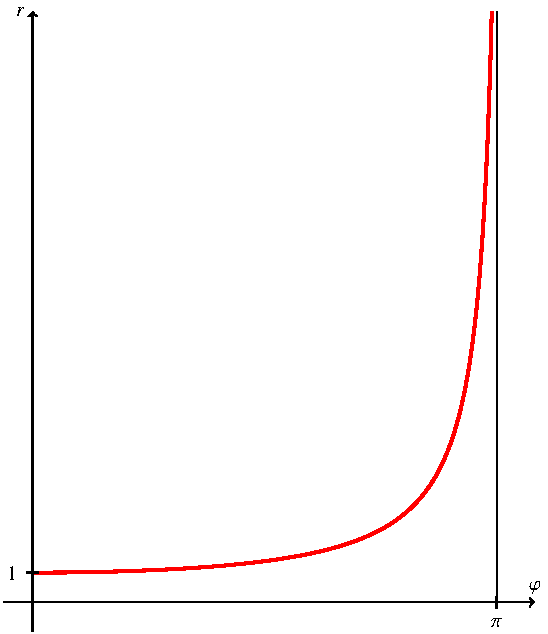
\includegraphics{chapters/tikz/lichtablenkung.pdf}
\caption{Die Lösung der Differentialgleichung~\eqref{skript:schwarzschild:udgl}
wächst in der Nähe des Ablenkungswinkels über alle Grenzen.
\label{skript:schwarzschild:abbildung:rphi}}
\end{figure}
Leider eignet sich die Differentialgleichung~\eqref{skript:schwarzschild:udgl}
nicht wirklich zur Berechnung des Ablenkungswinkels.
Schuld daran ist die Singularität, in der Nähe des Ablenkungswinkels
wächst $r(\varphi)$ über alle Grenzen, wie
Abbildung~\ref{skript:schwarzschild:abbildung:rphi} zeigt.

\subsection{Differentialgleichung für den Winkel}
Genau auf dem gleichen Weg wie wir eine Differentialgleichung für $r(\varphi)$
abgeleitet haben, können wir auch eine Differentialgleichung für
$\varphi$ als Funktion $r(\varphi)$ von $\varphi$ herleiten.
Dazu beachten wir, dass
\begin{align*}
\frac{d\varphi}{dr}&=\frac{\dot \varphi(s)}{\dot r(s)}
\qquad\text{und}
\\
\frac{d^2\varphi}{dr^2}
&=
\frac{\ddot\varphi(s)\dot r(s)-\ddot r(s)\dot\varphi(s)}{\dot r(s)^3}
\end{align*}
und setzen wie vorhin die bekannten Ableitungen $\ddot r(s)$ und
$\ddot\varphi(s)$ ein.
Wir erhalten
\begin{align*}
\frac{d^2\varphi}{dr^2}
&=
-\frac{2}{r}\frac{d\varphi}{dr}
-\frac{2r-3r_g}{2}\biggl(\frac{d\varphi}{dr}\biggr)^3
%\\
%&=
%-{{4\,\left({{d}\over{d\,s}}\,\varphi\left(s\right)\right)\,\left(
% {{d}\over{d\,s}}\,r\left(s\right)\right)^2+\left(2\,r^2\left(s
% \right)-3\,{\it rg}\,r\left(s\right)\right)\,\left({{d}\over{d\,s}}
% \,\varphi\left(s\right)\right)^3}\over{2\,r\left(s\right)\,\left({{d
% }\over{d\,s}}\,r\left(s\right)\right)^3}}
\end{align*}
Auch hier kann man mit $u=r/r_g$ wieder einen dimensionslosen Parameter
einführen, die Differentialgleichung vereinfacht sich dann zu
\begin{equation}
\frac{d^2\varphi}{du^2}
=
-\frac2{u}\frac{d\varphi}{du} -\frac{2u-3}2\biggl(\frac{d\varphi}{du}\biggr)^3.
\label{skript:schwarzschild:phidgl}
\end{equation}
Für diese Differentialgleichung ist es unproblematisch, die
Integration auch für grosse Werte von $u$ durchzuführen.

Die Differentialgleichungen
\eqref{skript:schwarzschild:udgl}
und
\eqref{skript:schwarzschild:phidgl}
können in Kombination dazu verwendet werden, den Ablenkungswinkel
numerisch zu berechnen.
Dazu verwendet man erst die Differentialgleichung
\eqref{skript:schwarzschild:udgl}
mit Anfangsbedingung
\begin{equation*}
\begin{aligned}
u(0)&=r/r_g,
\qquad&\qquad
u'(0)&=0.
\end{aligned}
\end{equation*}
bis zum $\varphi$-Wert $\varphi=\frac{\pi}4$.
Anschliessend kann man die
Differentialgleichung~\eqref{skript:schwarzschild:phidgl}
\begin{equation*}
\begin{aligned}
\varphi\biggl(u\biggl(\frac{\pi}2\biggr)\biggr)&=\frac{\pi}2,
\qquad&\qquad
\varphi'\biggl(u\biggl(\frac{\pi}2\biggr)\biggr)&=\frac1{u(\frac{\pi}2)}
\end{aligned}
\end{equation*}
bis zu einem sehr grossen Radius integrieren. 
Der Wert von $\varphi(u)$ strebt dabei gegen einen Wert
$\varphi_\infty>\frac{\pi}2$, der Ablenkungswinkel kann daraus als
\[
\alpha
=
(2\varphi_\infty - \pi)
\]
berechnet werden.
Das File \texttt{lichtablenkung.m} im Repository zeigt, wie dies mit
Octave gemacht werden kann.



